%% 5-minute presentation (about 9 slides, ~35 s each).  Build: scripts/run.sh docs   or   pdflatex slides.tex
\documentclass[aspectratio=169,11pt]{beamer}
\usetheme{Madrid}
\usecolortheme{seahorse}
\usepackage[T1]{fontenc}
\usepackage{tikz}
\usetikzlibrary{positioning,arrows.meta}
\usepackage{booktabs}
\newcommand{\code}[1]{\texttt{\small #1}}
\setbeamertemplate{navigation symbols}{}
\title{Multi-client Chat Application}
\subtitle{Project 9 --- Java client--server chat with groups, history and profiling}
\author{Mahesh \and Shravan \and Rajiv \and Shubham \and Divya}
\institute{IIT Dharwad}
\date{16 November 2026}

\begin{document}
\begin{frame}\titlepage\end{frame}

% 1 (30 s)
\begin{frame}{What we built}
\begin{itemize}
\item One \textbf{server} for many users at the same time
\item Two clients: \textbf{console} and \textbf{GUI window}
\item Register / login with \textbf{protected passwords}
\item \textbf{Public}, \textbf{private} and \textbf{group} messages with time stamps
\item \textbf{History}, saved users and groups, \textbf{server log}
\item Works across PCs on the same network (use the server's IP)
\end{itemize}
\end{frame}

% 2 (40 s)
\begin{frame}{How it is built}
\centering
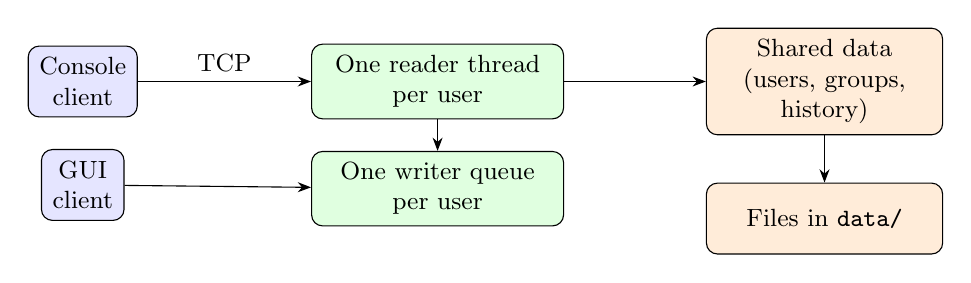
\begin{tikzpicture}[font=\small,>=Stealth,box/.style={draw,rounded corners,align=center,minimum height=9mm,inner sep=4pt}]
\node[box,fill=blue!10] (c) {Console\\client};
\node[box,fill=blue!10,below=4mm of c] (g) {GUI\\client};
\node[box,fill=green!12,right=22mm of c,minimum width=32mm] (r) {One reader thread\\per user};
\node[box,fill=green!12,below=4mm of r,minimum width=32mm] (w) {One writer queue\\per user};
\node[box,fill=orange!15,right=18mm of r,minimum width=30mm] (s) {Shared data\\(users, groups,\\history)};
\node[box,fill=orange!15,below=6mm of s,minimum width=30mm] (f) {Files in \code{data/}};
\draw[->] (c)--node[above]{TCP}(r); \draw[->] (g)--(w); \draw[->] (r)--(s); \draw[->] (s)--(f); \draw[->] (r)--(w);
\end{tikzpicture}

\vspace{2mm}
\small Slow disk or slow client never blocks the others: file writing runs in a background thread.
\end{frame}

% 3 (35 s)
\begin{frame}{Commands}
\small
\begin{tabular}{@{}ll@{}}
\toprule
\code{text} & message to everyone\\
\code{/msg bob hi} & private message\\
\code{/g team hello} & group message\\
\code{/group create | join | leave | list | mine | members} & manage groups\\
\code{/users}, \code{/history 20} & who is online, last messages\\
\bottomrule
\end{tabular}

\vspace{3mm}
\textbf{GUI:} click a person or group, then just type --- the GUI adds the command itself.
\end{frame}

% 4 (30 s)
\begin{frame}{Safe and reliable}
\begin{itemize}
\item Passwords are \textbf{salted and hashed} (PBKDF2), never stored as text
\item Thread-safe data structures: no two users can get the same name
\item Groups, users and history \textbf{survive a restart}
\item Everything that happens is written to \code{server.log}
\end{itemize}
\end{frame}

% 5 (35 s)
\begin{frame}{Automation and testing}
\begin{itemize}
\item \code{scripts/run.sh} --- build, start server / client / GUI
\item \code{scripts/test.sh} --- starts a server, runs \textbf{20 checks} (incl. restart), all pass
\item \code{scripts/profile.sh} --- profiling in one command
\item Tests found \textbf{3 real bugs}: groups lost after restart, a login race with 50 users, wasted hashing
\end{itemize}
\end{frame}

% 6 (50 s)
\begin{frame}{Profiling: time of each method}
Like \code{gprof}: calls, total and average time per method (\code{-Dprofile=true}).

\vspace{2mm}
\small
\begin{tabular}{@{}lrrr@{}}
\toprule
Method & Calls & Total (ms) & Avg (ms)\\
\midrule
\code{register} (hashing) & 22 & 51\,706 & 2\,350\\
\code{publicMessage} & 10\,020 & 22\,019 & 2.20\\
\code{send} & 201\,134 & 8\,348 & 0.042\\
\code{storeMessage} & 10\,060 & 3\,355 & 0.33\\
\code{/history} & 20 & 87 & 4.3\\
\code{/group create} & 20 & 46 & 2.3\\
\code{/group join} & 20 & 5.3 & 0.26\\
\bottomrule
\end{tabular}
\end{frame}

% 7 (35 s)
\begin{frame}{What the profile tells us}
\begin{itemize}
\item \textbf{Password hashing is the slowest step} --- on purpose (protects stolen passwords)
\item \textbf{Chatting is cheap:} one message to 20 users $\approx$ 2\,ms, one delivery 0.04\,ms \\
 $\rightarrow$ about 8\,500 messages/s on a 2-core machine
\item \textbf{File work costs more than memory work} (group create, history) $\rightarrow$ background writer thread
\item A client that stops reading no longer blocks others (receiver got all 20\,000 messages instead of about 6\,800 with our first version)
\end{itemize}
\end{frame}

% 8 (45 s)
\begin{frame}{Live demo}
\begin{enumerate}
\item \code{scripts/run.sh server 5000}
\item Open GUI as \textbf{alice}, console client as \textbf{bob}
\item Public message $\rightarrow$ click bob $\rightarrow$ private message
\item Create group \texttt{team}, bob joins, group message
\item \code{/history}, then \code{scripts/test.sh} (all checks pass)
\item Show \code{docs/profiling/profile.txt}
\end{enumerate}
\end{frame}

% 9 (20 s)
\begin{frame}{Team and summary}
\small
\begin{tabular}{@{}ll@{}}
Mahesh & server, bash scripts, tests\\
Shravan & console client\\
Rajiv & GUI\\
Shubham & profiling\\
Divya & documentation (README, report)\\
\end{tabular}

\vspace{3mm}
All requirements met: many users, login, private and group chat, history, log, GUI, tests, profiling.

\textbf{Future work:} encrypted connection (TLS), login limits, database for history.

\begin{center}\Large Thank you --- questions?\end{center}
\end{frame}
\end{document}
